% Four content pages plus references; presentation follows the supplied UAV draft.
\documentclass[letterpaper,10pt]{article}
\usepackage[T1]{fontenc}
\usepackage{times}
\usepackage[left=0.8in,right=0.8in,top=0.85in,bottom=0.75in]{geometry}
\usepackage{amsmath,amssymb,booktabs,graphicx,caption,multicol}
\usepackage[hidelinks,pdfauthor={},pdftitle={Profiled Joint Subset Search for Sparse Equation Discovery from Noisy Trajectories}]{hyperref}
\captionsetup{font=small,labelfont=normalfont,labelsep=period}
\setlength{\parindent}{1em}
\setlength{\parskip}{0pt}
\setlength{\columnsep}{0.3in}
\setlength{\multicolsep}{4pt}
\setlength{\abovecaptionskip}{4pt}
\setlength{\belowcaptionskip}{3pt}
\newcommand{\lead}[1]{\par\smallskip\noindent\textbf{#1}\ }
\makeatletter
\renewcommand\section{\@startsection{section}{1}{\z@}{-2.1ex plus -0.4ex minus -0.2ex}{1ex plus 0.2ex}{\normalfont\large\bfseries}}
\renewcommand\subsection{\@startsection{subsection}{2}{\z@}{-1.8ex plus -0.3ex minus -0.2ex}{0.8ex plus 0.2ex}{\normalfont\normalsize\bfseries}}
\renewcommand\@seccntformat[1]{\csname the#1\endcsname.\quad}
\makeatother
\newcommand{\LorenzCoef}{0.66}
\newcommand{\LorenzShort}{0.038}
\newcommand{\LorenzLong}{0.600}
\newcommand{\LorenzExact}{1}
\newcommand{\RosslerCoef}{0.25}
\newcommand{\RosslerShort}{0.060}
\newcommand{\RosslerLong}{0.095}
\newcommand{\RosslerExact}{1}
\newcommand{\ChenCoef}{1.93}
\newcommand{\ChenShort}{0.008}
\newcommand{\ChenLong}{0.015}
\newcommand{\ChenExact}{1}
\newcommand{\LorenzEqX}{-10.084x +10.110y}
\newcommand{\LorenzEqY}{27.844x -0.989y -0.994xz}
\newcommand{\LorenzEqZ}{-2.668z +1.003xy}

\newcommand{\StlsqCount}{269}
\newcommand{\StlsqOurs}{784}
\newcommand{\SrthreeCount}{153}
\newcommand{\SrthreeOurs}{784}
\newcommand{\EsindyCount}{86}
\newcommand{\EsindyOurs}{257}
\newcommand{\PysrCount}{56}
\newcommand{\PysrOurs}{117}
\newcommand{\OdeformerCount}{2}
\newcommand{\OdeformerOurs}{257}

\raggedbottom
\raggedcolumns
\begin{document}
\begin{center}
{\large\bfseries Profiled Joint Subset Search (PJSS) for Sparse Equation Discovery\\from Noisy Trajectories\par}
\vspace{5pt}
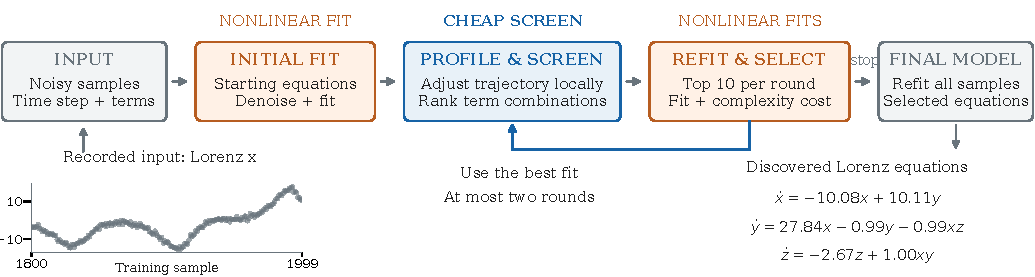
\includegraphics[width=\textwidth]{figures/architecture.pdf}
\captionof{figure}{System architecture. The blue stage cheaply estimates how well alternative equations could fit, allowing the trajectory to adjust. Only a shortlist receives full joint fits (orange). The trace and equations show the saved Lorenz example, with coefficients rounded for display.}
\label{fig:architecture}
\end{center}
\vspace{-4pt}

\begin{multicols}{2}
\begin{center}\textbf{\large Abstract}\end{center}
\noindent\textit{We study how to recover compact dynamical equations from noisy measurements using fewer expensive fitting steps. Profiled Joint Subset Search (PJSS) estimates the trajectory and equation together, screens alternative combinations of terms with a cheap approximation, and refits only a shortlist. The screen lets the trajectory adjust when the equation changes. On 80 paired tests, PJSS identifies the correct terms in 66 cases versus 61 for DEDi with complexity-based selection, at median runtimes of 14.4 and 5,930 seconds under the reported CPU/GPU setups. An operation-count study finds about 49 times fewer joint fits. Across 77 simulated systems, PJSS recovers the correct terms in 89.0\% of 6,160 tests. Reliable use on measured data remains open.}

\section{Introduction}
A noisy recording of a dynamical system may be explained by many equations. We want a small set of terms that captures its motion and predicts what happens next. The difficulty is choosing those terms while separating the underlying dynamics from measurement noise.

SINDy~\cite{sindy} selects terms from a predefined library by regression. Weak formulations~\cite{wsindy} reduce the need to differentiate noisy observations. SIDDS~\cite{sidds} and DEDi~\cite{dedi} estimate the equation and a clean trajectory together, but repeating this joint fit for many candidate equations is expensive.

PJSS aims to retain the benefit of joint fitting while reducing how often it is needed. It compares many candidates using a cheap score, then checks the most promising ones with full fits. We test recovery, runtime and the behaviour of the learned equations. The experiments use uniformly spaced measurements of every state variable, with the true equation contained in the candidate library.

\columnbreak
\section{Method}
\subsection{System overview}
Figure~\ref{fig:architecture} follows the measurements through the discovery process. Initial candidate equations provide a first estimate of the trajectory. A cheap screen then ranks alternative combinations of terms, allowing the trajectory to adjust with each change. A shortlist receives full joint fits. We compare their accuracy and size, use the best fit to update the screen, and finally refit the selected equation on all observations.

\subsection{Fitting the trajectory and equation}
Candidate terms are simple functions such as $1,x,y$ and $xz$. Their selected set is the \emph{support}; their coefficients determine how strongly they affect the motion. For observations $y_i\in\mathbb R^D$ at spacing $\Delta t$, write the dynamics as $\dot x=f(x)=C^\top\theta(x)$. The library $\theta$ has 20 terms up to cubic degree for three variables; higher-dimensional tests use quadratic terms.

For a given support, we adjust the coefficients $C$ and clean states $u$ together. A good fit must stay close to the measurements and follow the proposed equation. These two requirements give
\begin{equation}
\begin{aligned}
J_T(u,C)={}&\sum_{i\in T,j}\ell_2\!\left(\frac{u_{o(i),j}-y_{ij}}{\sigma_j}\right)\\[-2pt]
&+\sum_{k,j}\left(\frac{u_{k+1,j}-u_{k,j}-h f_j(m_k)}{\rho\sigma_j}\right)^2.
\end{aligned}\label{eq:objective}
\end{equation}
Here $\sigma_j$ is the estimated noise level. The clean trajectory uses a finer step $h=\Delta t/s$, with observation index $o(i)=is$ and midpoint $m_k=(u_k+u_{k+1})/2$. We set $\rho=0.03$ and use Huber loss $\ell_2(r)=r^2$ for $|r|\le2$, otherwise $4|r|-4$, to limit the influence of large observation errors. Coefficients outside the support stay zero. Every third observation (indices $2,5,8,\ldots$) is masked for model selection; $T$ contains the remainder.
\end{multicols}

\clearpage
\begin{multicols}{2}
\subsection{Screening alternative equations}
A new equation may need a different clean trajectory. Scoring it against the current trajectory alone could therefore reject a useful candidate. PJSS instead builds a quadratic approximation $Q$ to the joint fitting loss near the current fit. For coefficients $c=\operatorname{vec}(C)$ and current estimate $c^\star$, the \emph{profiled} score is
\begin{equation}
q(c)=\min_{\Delta u}Q(\Delta u,c-c^\star).
\label{eq:profile}
\end{equation}
Here $\Delta u$ is a local change to the trajectory. Computing it uses a linear solve, avoiding a new nonlinear fit for every candidate. Because this approximation is local, the shortlisted equations are subsequently checked by full fitting.

\subsection{Searching, refitting and selecting}
The screen compares combinations of terms, rather than choosing each term in isolation. For each equation, it considers zero to five terms and keeps two candidates at each size: 21,699 nonempty combinations for the three-variable cubic library. It combines equation replacements, ranks them by $\min q(c)+|S|\log(Dn)$, and jointly refits the ten best. Here $S$ is the support and $n$ the sample count. Search stops when the winner is unchanged or after two rounds.

The final comparison rewards fit quality while charging for extra terms. Its score adds the masked-observation loss and $\varphi\kappa\log(Dn)$ to $J_T$, where $\kappa$ counts terms with degree-dependent weights and $\varphi$ adjusts for correlated residuals. This heuristic follows the Bayesian information criterion (BIC)~\cite{bic}. Preprocessing also uses masked observations, so this check is not a test of unseen data. We refit the winning support on all samples, then with $\rho=0.001$, before returning coefficients in the original units.

\lead{Implementation.} We scale variables by their root-mean-square magnitude without centring. Smoothed observations initialise the trajectory; weak, hybrid and segment-based fits supply starting equations. Joint fitting uses banded Levenberg--Marquardt (40 iterations; relative cost tolerance $10^{-7}$). Noise levels and integration resolution are estimated from the data; an autoregressive option handles correlated errors. Full numerical settings are in the companion guide.

\section{Experimental setup}
\lead{Data and recovery.} We first test whether the method identifies the correct terms across different systems, record lengths and noise levels. The frozen \texttt{dysts} v0.96 benchmark~\cite{dysts} has 77 systems: 61 with three variables and terms up to cubic degree, and 16 with four to six variables and quadratic terms. Ten seeds, two lengths (500 and 2,000 samples) and four Gaussian noise levels (1, 5, 10 and 20\% of each coordinate's standard deviation) give 6,160 runs. Forty-nine systems are outside development; 28 overlap or share equation structure. Exact recovery requires all true terms and no extras in every equation; failed fits count as failures.

Reference trajectories use LSODA at $10^{-10}$ tolerances and sampling intervals adapted to each system's dominant frequency. Companion files preserve inputs, generation seeds and configurations. Frozen v1.0 benchmarks and v1.2 joint-method comparisons and illustrations are reported separately.

\lead{Baseline comparisons.} Regression and symbolic methods test term selection; DEDi tests the benefit of reducing repeated joint fits. Comparisons use the same inputs within each table row: 880 runs for standard regression, 294 for E-SINDy and ODEFormer, and 126 for PySR.

PySINDy~\cite{pysindy} estimates derivatives after smoothing. STLSQ, E-SINDy~\cite{esindy} and SR3~\cite{sr3} choose thresholds by five-fold regression-row cross-validation after full-record preprocessing. E-SINDy combines 20 fitted models. PySR~\cite{pysr} receives 60 seconds per equation and uses its ``best'' selector. ODEFormer~\cite{odeformer} uses 200 evenly spaced observations and its top candidate.

The core joint-method sample has 16 runs per condition in Table~\ref{tab:dedi}. A separate sample has 64 runs from 35 new systems, eight per noise/length cell. DEDi uses the authors' code with a banded solver, a full 35-setting grid and every third observation masked; we report validation and BIC selection. WSINDy uses MSTLS; ARGOS~\cite{argos} uses lasso and 200 bootstraps. The companion guide specifies all grids, archive indices and selection seeds. Selection never uses the true equation.
\end{multicols}
\vspace{-2pt}
\begin{center}
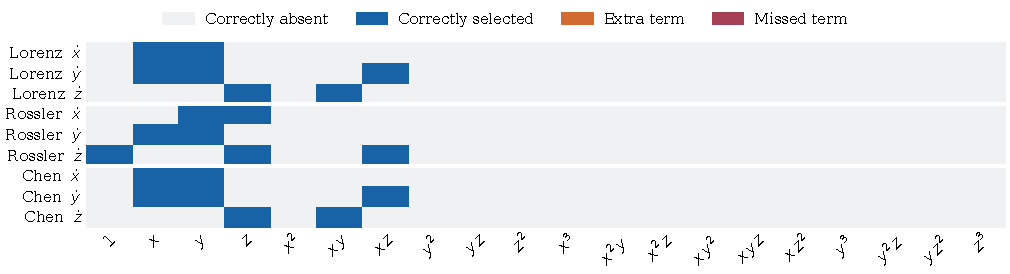
\includegraphics[width=0.95\textwidth]{figures/support.pdf}
\captionof{figure}{Recovered terms in the forecast examples. Each fit finds seven true terms, with no extras. Coefficient errors are \LorenzCoef\%, \RosslerCoef\% and \ChenCoef\% for Lorenz, R\"ossler and Chen. These selected examples do not measure overall recovery.}
\label{fig:support}
\end{center}

\clearpage
\section{Results and discussion}
\noindent\begin{minipage}[t]{0.478\textwidth}\vspace{0pt}
\lead{Recovery across systems.} PJSS recovers 89.0\% of all 6,160 runs and 85.3\% on the 49 new systems. Of 77 systems, 56 reach at least 90\% recovery and five fall below 50\% (Figure~\ref{fig:all-systems}). Small true terms and fast dynamics remain difficult.
\begin{center}\small
\captionof{table}{Exact recovery on paired \texttt{dysts} subsets. Each row uses the same inputs for both methods; PJSS is the frozen v1.0 result.}
\label{tab:standard}
\setlength{\tabcolsep}{3pt}
\begin{tabular}{@{}lrrr@{}}\toprule
Method / selection & Runs & Baseline & PJSS\\\midrule
STLSQ / CV & 880 & \StlsqCount & \StlsqOurs\\
SR3 / CV & 880 & \SrthreeCount & \SrthreeOurs\\
E-SINDy / CV & 294 & \EsindyCount & \EsindyOurs\\
PySR / best & 126 & \PysrCount & \PysrOurs\\
ODEFormer / top & 294 & \OdeformerCount & \OdeformerOurs\\\bottomrule
\end{tabular}
\end{center}
PJSS more often finds the exact polynomial terms than these baselines. This test measures equation structure, not every kind of modelling success: a different expression may predict the dynamics accurately and still count as non-exact.

\lead{Comparison with joint fitting.} Table~\ref{tab:dedi} tests whether the shorter search sacrifices accuracy relative to full-grid DEDi. The core result, 66/80 versus 61/80, does not establish that PJSS is more accurate: removing correlated-noise cases gives 56/64 for both. On new systems, PJSS alone succeeds in 15 cases and DEDi-BIC alone in three. Most of this advantage occurs at 1--5\% noise. These comparisons cover three-variable systems.
\begin{center}\small
\captionof{table}{Full-grid DEDi recovery. Each core row has 16 runs. Hard cases use Lorenz, Chen and R\"ossler; other core conditions draw from ten development systems. Short cases use 5--10\% noise; all other core rows use $n=2000$. New-system rows use both lengths.}
\label{tab:dedi}
\setlength{\tabcolsep}{4pt}
\begin{tabular}{@{}lrrr@{}}\toprule
Core condition & PJSS & DEDi val & BIC\\\midrule
Hard, 20\%, $n=2000$ & 15 & 13 & 15\\
White, 10--20\% & 14 & 14 & 14\\
AR(1), $a=0.8$ & 10 & 5 & 5\\
$t_3$, 10--20\% & 14 & 12 & 13\\
Short, $n=500$ & 13 & 11 & 14\\\midrule
All 80 runs & \textbf{66} & 55 & 61\\
\multicolumn{4}{@{}l}{\textit{Separate new-system sample (64 runs)}}\\
1--5\% noise (32) & 29 & 14 & 19\\
10--20\% noise (32) & 24 & 22 & 22\\\midrule
All 64 runs & \textbf{53} & 36 & 41\\\bottomrule
\end{tabular}
\end{center}

\lead{Contribution of each stage.} We compare variants on 576 paired runs (160 white, 89 correlated-noise, 40 hard and 287 \texttt{dysts}). Full PJSS finds the correct terms in 490. Holding the trajectory fixed during screening gives 480; choosing terms one at a time gives 462; omitting new proposals gives 458. All still perform nonlinear refits. Removing proposals loses 32 successes and gains none; trajectory adjustment adds 15 and loses five. Comparing term combinations supplies the larger gain, with a smaller benefit from profiling.
\end{minipage}\hfill
\begin{minipage}[t]{0.478\textwidth}\vspace{0pt}
\lead{Computation time.} PJSS takes a median \textbf{14.4\,s}, versus \textbf{5,930\,s} for full-grid DEDi (about 99 minutes), with 66/80 versus 61/80 correct models. The median-time ratio is \textbf{411} under the reported setups; the methods use different CPU/GPU resources.
\begin{center}\small
\captionof{table}{Recovery and runtime on the same 80 inputs, including model selection and excluding imports/data loading. PJSS and fast methods use one CPU core. DEDi uses a GPU shared by ten processes for 73 runs and CPUs for seven, on a loaded NVIDIA GB10 system.}
\label{tab:cost}
\setlength{\tabcolsep}{4pt}
\begin{tabular}{@{}lrr@{}}\toprule
Method / selection & Exact / 80 & Median s\\\midrule
WSINDy / MSTLS & 24 & 0.27\\
STLSQ / CV & 17 & 3.06\\
E-SINDy / CV & 17 & 59.8\\
ARGOS / lasso & 17 & 126\\
\textbf{PJSS v1.2} & \textbf{66} & \textbf{14.4}\\
DEDi / BIC & 61 & 5,930\\\bottomrule
\end{tabular}
\end{center}
Faster methods also involve an accuracy tradeoff. WSINDy, a checked port, takes only 0.27\,s but succeeds in 24/80 runs. Restricting DEDi to one or five settings gives 44/80 or 56/80 with BIC selection. We therefore use the full grid as the main joint-fitting comparison.

To separate the algorithm's work from hardware differences, we count joint fits. DEDi repeats them over 35 settings; PJSS uses cheap screening to limit them to a shortlist. PJSS requires a median of \textbf{21 joint fits} over 80 runs. Ten paired full-grid DEDi cases show a median \textbf{49-fold reduction in joint-fit count}, supporting fewer full fits as the source of the saving.
\begin{center}
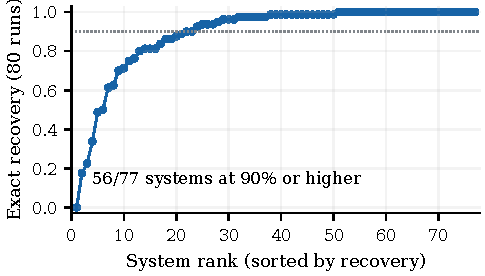
\includegraphics[width=\linewidth]{figures/recovery_systems.pdf}
\captionof{figure}{Recovery over all 77 systems. Each point uses 80 runs, sorted by exact-recovery rate. Difficult cases remain in the aggregate.}
\label{fig:all-systems}
\end{center}

\lead{Testing predictions.} Three v1.2 examples fit 2,000 observations at 10\% noise and predict 400 samples. Starting states use the final 40 training observations with coefficients fixed; no clean or future states enter. We use seed 20261105, burn-in 1,000 and $\Delta t=0.01,0.05,0.005$ for Lorenz, R\"ossler and Chen; LSODA uses $10^{-10}$ tolerances.
\end{minipage}

\clearpage
\subsection{Forecasts and recovered dynamics}
\begin{multicols}{2}
\lead{Forecast accuracy.} Finding the right terms does not ensure an accurate long forecast. All three examples recover the true terms, but their normalised root-mean-square error (RMSE) over 400 samples is \LorenzLong, \RosslerLong\ and \ChenLong\ for Lorenz, R\"ossler and Chen (Figure~\ref{fig:predictions}). Lorenz error rises from \LorenzShort\ over 100 samples to \LorenzLong\ over 400. The coefficients and starting state are still estimates, so equation recovery and prediction must be assessed separately. These examples illustrate behaviour, not a forecast ranking of methods.

\columnbreak
\lead{Long-run behaviour.} The attractor gallery compares the shapes traced by the learned and reference systems over time. Seven models find the correct terms and complete integration, including four outside development. Guckenheimer--Holmes and Atmospheric regime select incorrect terms and escape the integration bound (Figure~\ref{fig:attractors}). Saved-model pairs start at the same reference point to compare their dynamics without noisy-state initialisation. These selected examples show possible outcomes; they do not replace the 77-system benchmark.
\end{multicols}
\vspace{-4pt}
\begin{center}
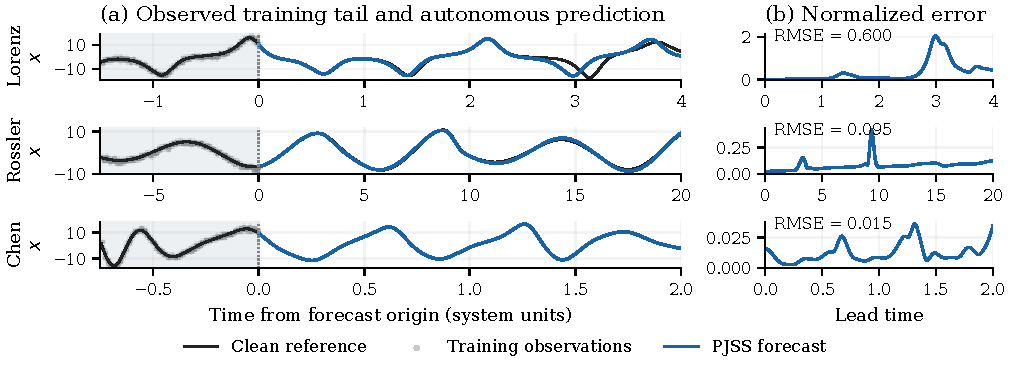
\includegraphics[width=0.96\textwidth]{figures/predictions.pdf}
\captionof{figure}{Forecasts (blue), clean reference (black) and observations (gray). Coordinate RMS errors use clean training standard deviations; annotations give 400-sample RMSE.}
\label{fig:predictions}
\end{center}
\vspace{-10pt}
\begin{center}
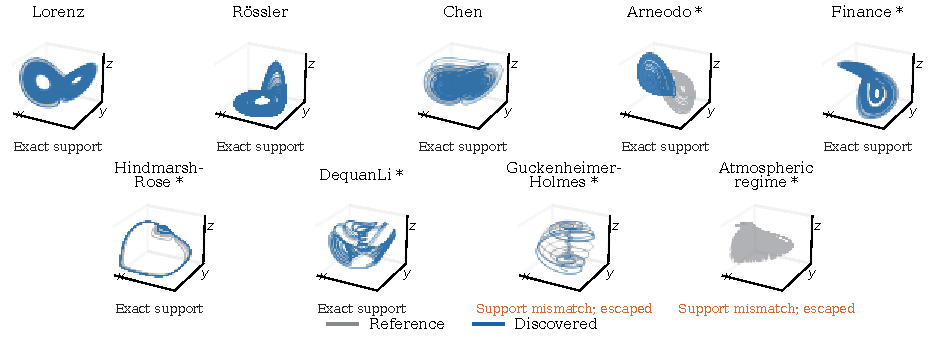
\includegraphics[width=0.93\textwidth]{figures/attractor_gallery.pdf}
\captionof{figure}{Reference (gray) and learned (blue) attractors. Stars mark systems outside development, using the lowest-index saved $n=2000$, 10\%-noise fit; the first three use fresh forecast models. Target: 8,000 samples after burn-in 1,000. Saved-model pairs use DOP853 at $10^{-8}/10^{-10}$ tolerances with a 20-times-reference-scale escape bound. Incomplete paths are labelled; off-view segments are masked.}
\label{fig:attractors}
\end{center}
\vspace{-12pt}
\noindent\begin{minipage}[t]{0.478\textwidth}\vspace{0pt}
\lead{Limitations and next steps.} Tests on measured pendulum data fail to recover the terms or meet forecast criteria, sometimes without warning. We have not established reliability when disturbances affect the dynamics or the library omits true terms. Future tests should compare forecasts and long-run statistics, beyond visual shape agreement.
\end{minipage}\hfill
\begin{minipage}[t]{0.478\textwidth}\vspace{0pt}
\section{Conclusion}
PJSS makes equation discovery faster by comparing many term combinations cheaply and fully fitting only a few. Searching combinations supplies the larger recovery gain; allowing the trajectory to adjust adds a smaller improvement. The main benefit is less computation, with accuracy depending on the comparison and noise conditions.
\end{minipage}

\clearpage
\begin{multicols}{2}
\begin{thebibliography}{12}
\small
\bibitem{sindy} S.~L. Brunton, J.~L. Proctor and J.~N. Kutz. Discovering governing equations from data by sparse identification of nonlinear dynamical systems. \emph{PNAS}, 113(15):3932--3937, 2016. \href{https://doi.org/10.1073/pnas.1517384113}{doi:10.1073/pnas.1517384113}.
\bibitem{wsindy} D.~A. Messenger and D.~M. Bortz. Weak SINDy: Galerkin-based data-driven model selection. \emph{Multiscale Modeling \& Simulation}, 19(3):1474--1497, 2021. \href{https://doi.org/10.1137/20M1343166}{doi:10.1137/20M1343166}.
\bibitem{sidds} J.~M. Hokanson, G.~Iaccarino and A.~Doostan. Simultaneous identification and denoising of dynamical systems. \emph{SIAM J. Scientific Computing}, 45(4):A1413--A1437, 2023. \href{https://doi.org/10.1137/22M1486303}{doi:10.1137/22M1486303}.
\bibitem{dedi} T.~Meissner and K.~Glasner. Simultaneous model discovery and state estimation under high data corruption. \emph{SIAM J. Applied Dynamical Systems}, 25(2):1439--1467, 2026. \href{https://doi.org/10.1137/24M1681008}{doi:10.1137/24M1681008}.
\bibitem{bic} G.~Schwarz. Estimating the dimension of a model. \emph{Annals of Statistics}, 6(2):461--464, 1978. \href{https://doi.org/10.1214/aos/1176344136}{doi:10.1214/aos/1176344136}.
\bibitem{dysts} W.~Gilpin. Chaos as an interpretable benchmark for forecasting and data-driven modelling. \emph{NeurIPS Datasets and Benchmarks}, 1, 2021. \href{https://arxiv.org/abs/2110.05266}{arXiv:2110.05266}.
\bibitem{pysindy} A.~A. Kaptanoglu et al. PySINDy: A comprehensive Python package for robust sparse system identification. \emph{J. Open Source Software}, 7(69):3994, 2022. \href{https://doi.org/10.21105/joss.03994}{doi:10.21105/joss.03994}.
\bibitem{esindy} U.~Fasel, J.~N. Kutz, B.~W. Brunton and S.~L. Brunton. Ensemble-SINDy: Robust sparse model discovery in the low-data, high-noise limit, with active learning and control. \emph{Proc. Royal Society A}, 478(2260):20210904, 2022. \href{https://doi.org/10.1098/rspa.2021.0904}{doi:10.1098/rspa.2021.0904}.
\bibitem{sr3} K.~Champion, P.~Zheng, A.~Y. Aravkin, S.~L. Brunton and J.~N. Kutz. A unified sparse optimization framework to learn parsimonious physics-informed models from data. \emph{IEEE Access}, 8:169259--169271, 2020. \href{https://doi.org/10.1109/ACCESS.2020.3023625}{doi:10.1109/ACCESS.2020.3023625}.
\bibitem{pysr} M.~Cranmer. Interpretable machine learning for science with PySR and SymbolicRegression.jl. \emph{arXiv preprint}, 2023. \href{https://arxiv.org/abs/2305.01582}{arXiv:2305.01582}.
\bibitem{odeformer} S.~d'Ascoli, S.~Becker, A.~Mathis, P.~Schwaller and N.~Kilbertus. ODEFormer: Symbolic regression of dynamical systems with transformers. \emph{ICLR}, 2024. \href{https://arxiv.org/abs/2310.05573}{arXiv:2310.05573}.
\bibitem{argos} K.~Egan, W.~Li and R.~Carvalho. Automatically discovering ordinary differential equations from data with sparse regression. \emph{Communications Physics}, 7:20, 2024. \href{https://doi.org/10.1038/s42005-023-01516-2}{doi:10.1038/s42005-023-01516-2}.
\end{thebibliography}
\end{multicols}
\end{document}
